\documentclass[a4paper, report, oneside, UKenglish]{memoir}


%% Title page
\usepackage{projectfp}


%% Silence warning about obsolete package
\usepackage{silence}
\WarningFilter{remreset}{The remreset package}


%% Encoding
\usepackage[utf8]{inputenx} % Source code
\usepackage[T1]{fontenc}    % PDF


%% Fonts and typography
\usepackage{lmodern}           % Latin Modern Roman
\usepackage[scaled]{beramono}  % Bera Mono (Bitstream Vera Sans Mono)
\renewcommand{\sfdefault}{lmss} % Latin Modern Sans Serif
\usepackage[final]{microtype}  % Improved typography
\renewcommand{\abstractnamefont}{\Large\sffamily\bfseries}           % Abstract
\renewcommand*{\chaptitlefont}{\Huge\bfseries\rmfamily\raggedright}  % Chapter
\setsecheadstyle{\Large\bfseries\sffamily\raggedright}               % Section
\setsubsecheadstyle{\large\bfseries\sffamily\raggedright}            % Subsection
\setsubsubsecheadstyle{\normalsize\bfseries\sffamily\raggedright}    % Subsubsection
\setparaheadstyle{\normalsize\bfseries\sffamily\raggedright}         % Paragraph
\setsubparaheadstyle{\normalsize\bfseries\sffamily\raggedright}      % Subparagraph
\setsecnumdepth{subsection}

\usepackage{geometry}

%% Mathematics
\usepackage{amsmath}
\usepackage{amssymb}   % Extra symbols
\usepackage{amsthm}    % Theorem-like environments
\usepackage{thmtools}  % Theorem-like environments
\usepackage{mathtools} % Fonts and environments for mathematical formulae
\usepackage{mathrsfs}  % Script font with \mathscr{}
\usepackage{physics}

%% Miscellanous
\usepackage{graphicx}  % Tool for images
\graphicspath{{figures/}}
\usepackage{babel}     % Automatic translations
\usepackage{csquotes}  % Quotes
\usepackage{textcomp}  % Extra symbols
\usepackage{listings}  % Typesetting code
\lstset{basicstyle = \ttfamily, frame = tb}
\usepackage{multirow}  % Multirow equations
\usepackage[table,xcdraw]{xcolor} % Color for tables
\usepackage{gensymb}   % Symbols
\usepackage[center]{caption}
\usepackage{parskip}
\usepackage[hidelinks]{hyperref} % Hide red boxes around links


%% Bibliography
\usepackage[style=ieee]{biblatex}
\usepackage{mathscinet}
% \usepackage[backend    = biber,
%             sortcites  = true,
%             giveninits = true,
%             doi        = false,
%             isbn       = false,
%             url        = false,
%             style      = alphabetic
%             citestyle  = numeric]{biblatex}
% \DeclareNameAlias{sortname}{family-given}
% \DeclareNameAlias{default}{family-given}
% \DeclareFieldFormat[article]{volume}{\bibstring{jourvol}\addnbspace#1}
% \DeclareFieldFormat[article]{number}{\bibstring{number}\addnbspace#1}
% \renewbibmacro*{volume+number+eid}
% {
%     \printfield{volume}
%     \setunit{\addcomma\space}
%     \printfield{number}
%     \setunit{\addcomma\space}
%     \printfield{eid}
% }
\bibliography{bibliography}
\addbibresource{bibliography.bib}

%% Cross references
%\usepackage{varioref}
%\usepackage[pdfusetitle]{hyperref}
%\urlstyle{sf}
%\usepackage[nameinlink, capitalize, noabbrev]{cleveref}
%\crefname{chapter}{Section}{Sections}

%% Delimiters
\DeclarePairedDelimiter{\paren}{\lparen}{\rparen}   % Parenthesis
\DeclarePairedDelimiter{\set}{\lbrace}{\rbrace} % Set
% \DeclarePairedDelimiter{\abs}{\lvert}{\rvert}   % Absolute value
% \DeclarePairedDelimiter{\norm}{\lVert}{\rVert}  % Norm


%% Operators
\newcommand{\diff}{\mathop{}\!\mathrm{d}}
\DeclareMathOperator{\im}{im}
% \DeclareMathOperator{\rank}{rank}
\DeclareMathOperator{\E}{E}
\DeclareMathOperator{\Var}{Var}
\DeclareMathOperator{\Cov}{Cov}

%% New commands for vectors
\newcommand{\ba}{\boldsymbol{a}}
\newcommand{\bD}{\boldsymbol{D}}
\newcommand{\x}{\boldsymbol{x}}
\newcommand{\bz}{\boldsymbol{z}}
\newcommand{\bdelta}{\boldsymbol{\delta}}
\newcommand{\btheta}{\boldsymbol{\theta}}
\newcommand{\bDelta}{\boldsymbol{\Delta}}
\newcommand{\bTheta}{\boldsymbol{\Theta}}


%% New commands for sets
\newcommand{\N}{\mathbb{N}}   % Natural numbers
\newcommand{\Z}{\mathbb{Z}}   % Integers
\newcommand{\Q}{\mathbb{Q}}   % Rational numbers
\newcommand{\R}{\mathbb{R}}   % Real numbers
\newcommand{\C}{\mathbb{C}}   % Complex numbers
\newcommand{\A}{\mathbb{A}}   % Affine space
\renewcommand{\P}{\mathbb{P}} % Projective space


%% Miscellanous
\renewcommand{\qedsymbol}{\(\blacksquare\)}
\setlength{\parindent}{0pt} % Indent before each paragraph
\setlength{\parskip}{7pt}   % Space between paragraphs


\title{ML Project}
\author{Andrea Bellés Ferreres \newline Arnau Ochoa Bañuelos}
\supervisor{Carl Milner\newline Heekwon No}

\begin{document}

\projectfrontpage

\newpage
\begin{abstract}
\noindent

\end{abstract}

\newpage
\begin{KeepFromToc}
    \tableofcontents
\end{KeepFromToc}

\newpage
\chapter{Introduction}\label{ch:intro}
Global Navigation Satellite System (GNSS) refers to a constellation of satellites transmitting signals from space that provide positioning and timing data to GNSS receivers. Then, these receivers use the data to determine the their own location.

Satellite-based systems present many advantages with respect to other positioning systems, such that global coverage and long-term accuracy with errors limited to a few meters \cite{groves}, considering a stand-alone standard GNSS receiver. Consequently, this type of navigation systems are being employed in a wide range of applications, not only for positioning purposes, but also to improve traffic flow, assist in civil protection and rescue operations, and research on subjects such that geodesy, meteorology and surveying, among many others \cite{EGSAwebsite}. 

The rising demand of real-time information entiles the use of GNSS in many fields, such as the European railway network. In December 2019, the European Commission invested in the development of a new research project, known as Certifiable Localisation Unit with GNSS  (CLUG) in the railway environment, within the framework of the Horizon 2020 programme. This EU project aims to assess the feasibility of a failsafe on-board multi-sensor localisation unit using GNSS, track maps and a minimal number of reference points \cite{CORDISwebsite}. It will also review the use of an on-board continuous localisation system that provides information on location, speed and other dynamics of the train \cite{CORDISwebsite}. The future purpose is the development of train digitalisation and automation. 

In addition to the coordinate collaboration of multiple railway companies, railway signalling industries and navigation specialists \cite{CORDISwebsite}, part of this project is carried out in the École Nationale de l'Aviation Civile (ENAC). It is proposing to develop an innovate model of the local errors impacting the GNSS receiver. Besides that, ENAC's role consists in helping to develop the end-to-end integrity concept including an assesment of the error and fault models.  

In order to support this work, ENAC is collecting its own data within the complex urban environments that the CLUG project is addressing by using the "Jumpy" research vehicle of the institution.

As part of the work developed by ENAC, this project aims to contribute to the development of different regression techniques to generate a model for the local errors. Different fitting algorithms have been implemented for this modelling: a Matlab fitting function, Gradient Descent (GD) and Neural Networks (NN). Each of them will be further detailed in the following chapters. 

% search references of the use of neural networks for estimating the quality of the signal (multipath, overall error, etc)

%%% todo: resume of what are we going to do mentioning where it is going to be explain:
%%%% Ex: Throughout this document we will analyse.... blablabla in chapter 1.... sth like this
%%Throughout this project, regression models have been considered in order to solve a predictive problem with regard to the modelling of local errors present in a set of features, which have been provided by the supervisors of this project, and the corresponding polynomial relationship of those features which best captures the error distribution

% s'han desenvolupat els metodes fent servir MATLAB fitting, pero despres el analisis principal es amb mes features. Mes que res perque 
% 1. sabem (o intuim bastant) que modelar el mp amb cno i elev es dificil, pq no ens donen prou info
% 2. la gracia de fer servir NN es poder analitzar mes features de les que analitzaries amb altres metodes (i trobar patrons mes complexos), del que ho faries amb un LS o GD. (a part del aprenentatge automatic i tal) 
% crec que aquest es com el main purpose del treball, rollo la hipotesi que tenim i tal

        
% ...

% Fitting (o regression o whatever)
%     matlab fitting -> first reference
%     gradient descent -> interesting method (?), reference for NN
%     neural networks -> expected to have better performance since it allows to find more complex relations between data (aprox)

%==================================================================================================================
\chapter{Data analysis}\label{ch:data_analysis}
% explain the concept of features

% Introduction about the data we are using
%   Two stages in terms of data:
%       First we used Pseudo-range Error, CN0 and elevation to develop the algorithms and get familiar with (data?). Also, the other data was not available yet.
%       Later, we obtained more data 


% Data analysis and preparation
%     - Data analysis:
%         

% Data preparation
%   remove outliers
%   remove invalid data (CN0 = 0, nan)
%   distribution, comparation with gaussian, Kurtosis? etc

% Data analysis

%==================================================================================================================
\chapter{Fitting}\label{ch:fitting}

\section{MATLAB fitting}

Regression analysis is a statistical tool which enables to estimate the relationship between an output variable and one or several input variables. Therefore, it helps to depict the causal effect of certain parameters upon other ones \cite{IntroToRegresAna}. Regression models have been long used in many fields, such as economics, medicine or chemistry, principally for purposes related to predict, forecast and estimate values between observed data points \cite{MathWorksRegression}.  

Throughout this project, regression models have been considered in order to estimate the distribution of the errors present in the aforementioned features. This section focuses on nonlinear regression of the mean and standard deviation (STD) of the Multipath Error (PRE) as a function of elevation and Carrier-to-Noise (CN0) by using the Curve Fitting Toolbox\textsuperscript{\tiny\texttrademark} software developed for MATLAB\textsuperscript{\tiny\textregistered}. The aim of using this estimation technique is to provide a first intuition about the error modelling of the data initially provided. In addition, this fitting is a tool used to provide a reference of the resulting error model in order to compare the performance with other methods. Thus, the algorithms implemented can be validated as it was assumed that the results must be improved using more advanced techniques, such as Gradient Descent (GD) or Neural Networks (NN). 

The Curve Fitting Toolbox\textsuperscript{\tiny\texttrademark} includes a set of functions and utilities which allow to perform a regression by fitting a curve or surface to the data through linear and nonlinear models, or custom equations \cite{MathWorksRegression}. In consequence, fitting requires to define a parametric model which establishes a relation between a set of training data and the output variable using a number of coefficients, so that the output continuous-valued parameter can be predicted. 

Fitting a curve or a surface mainly depends on the number of features available. Thus, the measurement model is build in accordance with the number of features. In our case, there are two possible options: selecting one or two features. As a result, the algorithm fits a curve when one feature is selected, otherwise it fits a surface.

This software uses the Least Squares (LS) regression method to fit the data, which consists in obtaining the best estimator by minimizing the sum of squared residuals. For this fitting, two different nonlinear measurements models are considered: polynomial and exponential. 

Given a general nonlinear function $h$ to represent the measurement model for one feature, such that
\begin{equation}
    y = h(x,p) + \epsilon
\end{equation}
where $y$ is the output variable, $x$ is the input variable, $p$ corresponds to the coefficients of the model and $\epsilon$ corresponds to the error. Consequently, from the general model, it is possible to go into detail with respect to the aforementioned nonlinear models. 

On one side, a polynomial measurement model for a single feature is assumed, such that
\begin{equation}
    y_k = \sum\limits_{i=i}^{n+1} p_{i}x^{n+1-i},  \;\;\mbox{for}\; k = 1,...,M
\end{equation}

where $n+1$ is the order of the polynomial, which indicates the number of coefficient to be fit, and $n$ is the degree of the polynomial, which gives the highest power of the predictor variable. In addition, $x = [x_1,...,x_N]$ is the set of N know inputs, $y = [y_1,...,y_M]$ is the set of M observations and $p = [p_1,...,p_N]$ corresponds to the coefficient estimates.

The degree of the polynomial and, thus, the number of coefficients to be estimated may be modified according the problem requirements or needs. 
An example of the resulting model may be the following
\begin{equation}
\begin{split}
    y_k &= p_{1}x^{2} + p_{2}x + p_3,    \;\;\mbox{for}\; k = 1,...,M
\end{split}
\end{equation}

However, the toolbox allows to fit curves up to polynomials of degree 9, if desired. 

The main advantages of polynomial fits include reasonable flexibility for data that is not too complicated, and they are linear, which simplifies the fitting process \cite{MathWorksRegression}. However, high-degree models can become unstable and diverge extensively outside the data range \cite{MathWorksRegression}. 
% Explaining why polynomial here?

On the other side, it is also presented the one-term exponential measurement model, such that 
\begin{equation}
    y_k = p_{1}e^{p_{2}x_{k}},  \;\;\mbox{for}\; k = 1,...,M
\end{equation}
%% Explain why using exponential, advantages? disadvantages?

After introducing the measurements models implemented for one feature, the measurements models for two features are presented hereunder.

The nonlinear $h$ can be expressed as a function of two variables:
\begin{equation}
    y = h(x_{1},x_{2},p) + \epsilon
\end{equation}
where $y$ is the output variable, $x_{1}$ and $x_{2}$ are the features, $p$ corresponds to the coefficients of the model and $\epsilon$ corresponds to the error. 

This model can also be further detailed considering the polynomial model. It is important to notice that, in this case, the exponential model is not available for surface fitting in the MATLAB toolbox used. In consequence, the estimation of the mean and STD with two features has been carried out has been carried out using only a polynomial hypothesis.

An example of a polynomial measurement model with two features can be as follows:
\begin{equation}
\begin{split}
    y_k &= p_{00} + p_{10}x_{1} + p_{01}x_{2} + p_{11}x_{1}x_{2} + p_{20}x^{2}_{1} + p_{02}x^{2}_{2},    \;\;\mbox{for}\; k = 1,...,M
\end{split}
\end{equation}

In this case, the toolbox allows to fit a surface using polynomials up to degree 5. 

Once the measurement model is defined, it is time to introduce the main core of the fitting algorithm, which is the nonlinear Least Squares method. As it has been previously stated, the goal of the LS is to minimize the sum of squared residuals $r_k$ (SSR), so that the coefficient estimates $\hat{p}$ are obtained.
\begin{equation}\label{eq:SSR}
    SSR(p) = \sum\limits_{k=1}^{M}{r}_{k}^{2} = \sum\limits_{k=1}^{M}(y_k - \hat{y}_k)^2 = \sum\limits_{k=1}^{M}(y_k - \sum\limits_{i=i}^{n+1} p_{i}x^{n+1-i})^2
\end{equation}

Equivalently, equation \eqref{eq:SSR} can be expressed in a matrix way:
\begin{equation}
    SSR(p) = \sum\limits_{k=1}^{M}(Y - x_{i}p)^2 = (Y - xp)^T(Y - xp)
\end{equation}

Equation \eqref{eq:SSR} represents the cost function of the model, which gives a good measure of how well the particular model fits the dataset \cite{MachLearnRefined}. In order to obtain the minimum $\hat{p}$, this function must be minimized, which is accomplished by applying differentiation and scaling techniques:
\begin{equation}
\begin{split}
    \left.-\frac{1}{2}\pdv{(SSR(p))}{p_{j}}\right|_{\substack{\hat{p}}} &= x^{T}(Y - xp) = 0
\end{split}
\end{equation}

The final expression of the estimates is as follows:
\begin{equation}\label{eq:estimatorLS}
\begin{split}
    \hat{p} = (\textbf{X}^{T}\textbf{X})^{-1}\textbf{X}^{T}Y = \textbf{S}Y\\
\end{split}
\end{equation}

where $\textbf{X}$ is the matrix of features, $\textbf{W}$ corresponds to the weight matrix and $\textbf{S}$ is called generalized inverse or pseudoinverse.

As nonlinear models are more difficult to fit than the linear ones, an iterative approach is required to perform instead of simple matrix techniques \cite{MathWorksRegression}. So, it is necessary to provide an initial estimate of the coefficients, which is set to [0,0] in this case. Hence, the function produces a initial fitted curve for the current set of coefficients. Then, the software adjusts the coefficients and determine whether the fit improves. Finally, it iterates the process until the fit reaches the specified convergence criteria \cite{MathWorksRegression}. 

In addition to the nonlinear LS, we have also implemented a nonlinear Weighted Least Squares (WLS). This variant of the LS is specially useful when the assumption such that the output data has constant variance is no longer fulfilled. Therefore, the WLS is a powerful tool to improve the fit, which consists in including additional weights in the fitting process in order to give more importance (more weight) to the high-quality data, which will have a greater impact on the final coefficient estimates. 

Due to the weights, defined as $w_{k}$, the expression of the SSR in equation \eqref{eq:SSR} results in
\begin{equation}\label{eq:SSR}
    SSR(p) = \sum\limits_{k=1}^{M}w_{k}{r}_{k}^{2} = \sum\limits_{k=1}^{M}w_{k}(y_k - \hat{y}_k)^2
\end{equation}

Accordingly, 
\begin{equation}
    SSR(p) = (Y - xp)^T\textbf{W}(Y - xp)
\end{equation} 

where $\textbf{W} = \frac{1}{h(x,p)}\textbf{I}$, considering $\textbf{I}$ an identity matrix. 

So, the formulation of the estimates is modified such that
\begin{equation}\label{eq:estimatorWLS}
\begin{split}
    \hat{p} = (\textbf{X}^{T}\textbf{W}\textbf{X})^{-1}\textbf{X}^{T}\textbf{W}Y\\
\end{split}
\end{equation}

\subsection{Architecture of our curve fitting}

Once the fundamentals of the curve fitting are understood, we can proceed to introduce the structure of the algorithm implemented in order to clarify the steps carried out for the present regression method.

First of all, as it has been mentioned previously, the fitting is conducted in order to obtain the coefficient estimates of the mean ($\mu$) and STD ($\sigma$) of the PRE. To achieve this objective, it is important to differentiate both types fittings. 

Regarding to the mean fitting, the input parameters of the function correspond to the given features and the observed data points. In this case, the features are the elevation and CN0 and the observed data corresponds to the PRE. The magnitude of the PRE depends on many factors and, among them, the aforementioned ones are present. Hence, both inputs are necessary to perform the LS regression and, therefore, obtaining the output, which corresponds to the estimate of the variable being measured: the mean of the PRE.  

As a quick reminder of the previous chapter \ref{ch:data_analysis}, at this point, the data has already been processed in order to discard invalid or undesired values. 

In this sense, the procedure followed for the computation of the mean fitting can be resumed with the following steps:
\begin{enumerate}
    \item Define fitting options,
    \item Introduce features and observed data points,  
    \item Apply curve fitting function to estimate the coefficients of the model,
    \item Evaluate the regression model with the input data and the coefficients estimates,
    \item Compute Root Mean Squared Error (RMSE). 
\end{enumerate}

Regarding the RMSE, it represents a measure of the error made by the model in predicting the observed data. The RMSE of predicted values is computed as follows:

\begin{equation}
    RMSE = \sqrt{\frac{\sum\limits_{k=1}^{M}{r}_{k}^{2}}{M}} = \sqrt{\frac{\sum\limits_{k=1}^{M}{r}_{k}^{2}}{M}} = \sqrt{\frac{\sum\limits_{k=1}^{M}(y_k - \hat{y}_k)^2}{M}} 
\end{equation}

This computation is equivalent for the mean and the STD estimation, as well as for the WLS. The only consideration is that the observed values $y$ and predicted ones $\hat{y}$ represent different parameters in each case.  
 
Hence, RMSE is a useful tool to get a measure of the spread of the $y$ values about the predicted $\hat{y}$ values \cite{StanfordRMSE}. As the effect of each error on the RMSE is proportional to the size of the squared error, then larger errors have a disproportional impact on the RMSE, leading to extremely large errors. As a result, RMSE is very sensitive to outliers. In this case, the RMSE is a parameter used to analyze and compare the performance of the different regression models implemented in this project.   

On the other hand, the fitting of the STD carries out the estimation of the error of the observed variables, in this case the PRE, with respect to the features provided. This particularity requires a previous step in comparison with the mean fitting. As the regression is applied to the error of the observed parameter instead of the total value, then the residuals are additionally computed prior to perform the fitting.  

So, the input variable or vector corresponds to:
\begin{equation}\label{eq:inputstd}
\begin{split}
    r_{k,\sigma} = |y_k - \hat{y}_{k,\mu}| = |y_k - h(x_{k},\hat{p}_{k,\mu})| = |y_k - x_{k}p_{k,\mu}|\\
\end{split}
\end{equation}

Once the computation is made according to equation \eqref{eq:inputstd}, the same steps as previously stated for the mean fitting are followed. 

Finally, this procedure is repeated for the nonlinear WLS regression method, in which the computation of the weights must be taken into consideration before the fitting for both mean and STD. 

% The main reason behind the decision to select a polynomial model is the distribution of the data provided. According to the results presented in chapter \ref{ch:data_analysis}, 

\section{Gradient descent}

Gradient descent is an optimization algorithm, which has become very popular in the recent years as it is widely used for training machine learning models. However, it was developed by Lous Augustin Cauchy in his \textit{Compte Rendu à l’Académie des Sciences} of October 18, 1847 \cite{cauchy}. 



\section{Neural Network}
% Introduction
The concept of Artificial Neural Networks, also known just as neural networks, was first introduced in the early 1940s by McCullock and Pitts, who theorized about a computational model for artificial intelligence which was inspired on the neural networks in the brain \cite{mcculloch_logical_1943}. Later, in 1958, Rosenblatt developed the perceptron which can be considered as the equivalent of a neuron in Artificial Neural Networks \cite{rosenblatt_perceptron_1958}. The perceptron allowed to learn from a set of example data and later perform binary classification of new examples. In 1969 it was demonstrated that perceptrons were incapable of performing non-linear classifications such as performing the logical XOR operation \cite{minsky69perceptrons}. The development of the backpropagation algorithm in 1975 renewed the interest in neural networks because it allowed to train multiple-layer perceptrons \cite{werbos}. These were networks of various neurons that allowed the learning of non-linear functions. Even then, neural networks were rarely used due to the high computational complexity and the large amounts of data that they required. An increase in transistor count and a latter raise in the use of GPUs have bring back to life the neural networks, also the Internet explosion allowed a much easier collection of large amounts of data, which are needed to train neural networks \cite{aggarwal_neural_2018}.

Lately, neural networks have outperformed other regression algorithms in many complex problems and have also empowered new and unforeseen applications such as vehicle control \cite{BojarskiTDFFGJM16}, image recognition \cite{hijazi2015} or medical diagnosis \cite{AMATO201347}.

\subsection{Model representation}
The basic element in a neural network is called neuron. A neuron is nothing more that an element that takes some weighted inputs, adds them to obtain $z$ and maps the result to another value, $g(z)$, which is the output. The function $g(z)$ is called \textit{activation function} and it is the main characteristic of the neuron. The behavior of a neuron is expressed as

\begin{equation}
    g(z) = g(\btheta^T\boldsymbol{x})
\end{equation}

where $\x = [x_0, x_1, x_2, ..., x_n]^T$ are the input values $x_0 = 1$, and $\btheta = [\theta_0, \theta_1, \theta_2, ..., \theta_n]$ are the weights assigned to these input values. The idea of this model is that, given the correct weights to the input values and the right activation function, it will estimate a value $y^{(i)}$ which depends on the input $\boldsymbol{x^{(i)}}$ as $h_\theta(\boldsymbol{x^{(i)}})$. This neuron can be represented with the diagram in Fig. \ref{fig:neuron_diag}. 

\begin{figure}[ht]
    \centering
    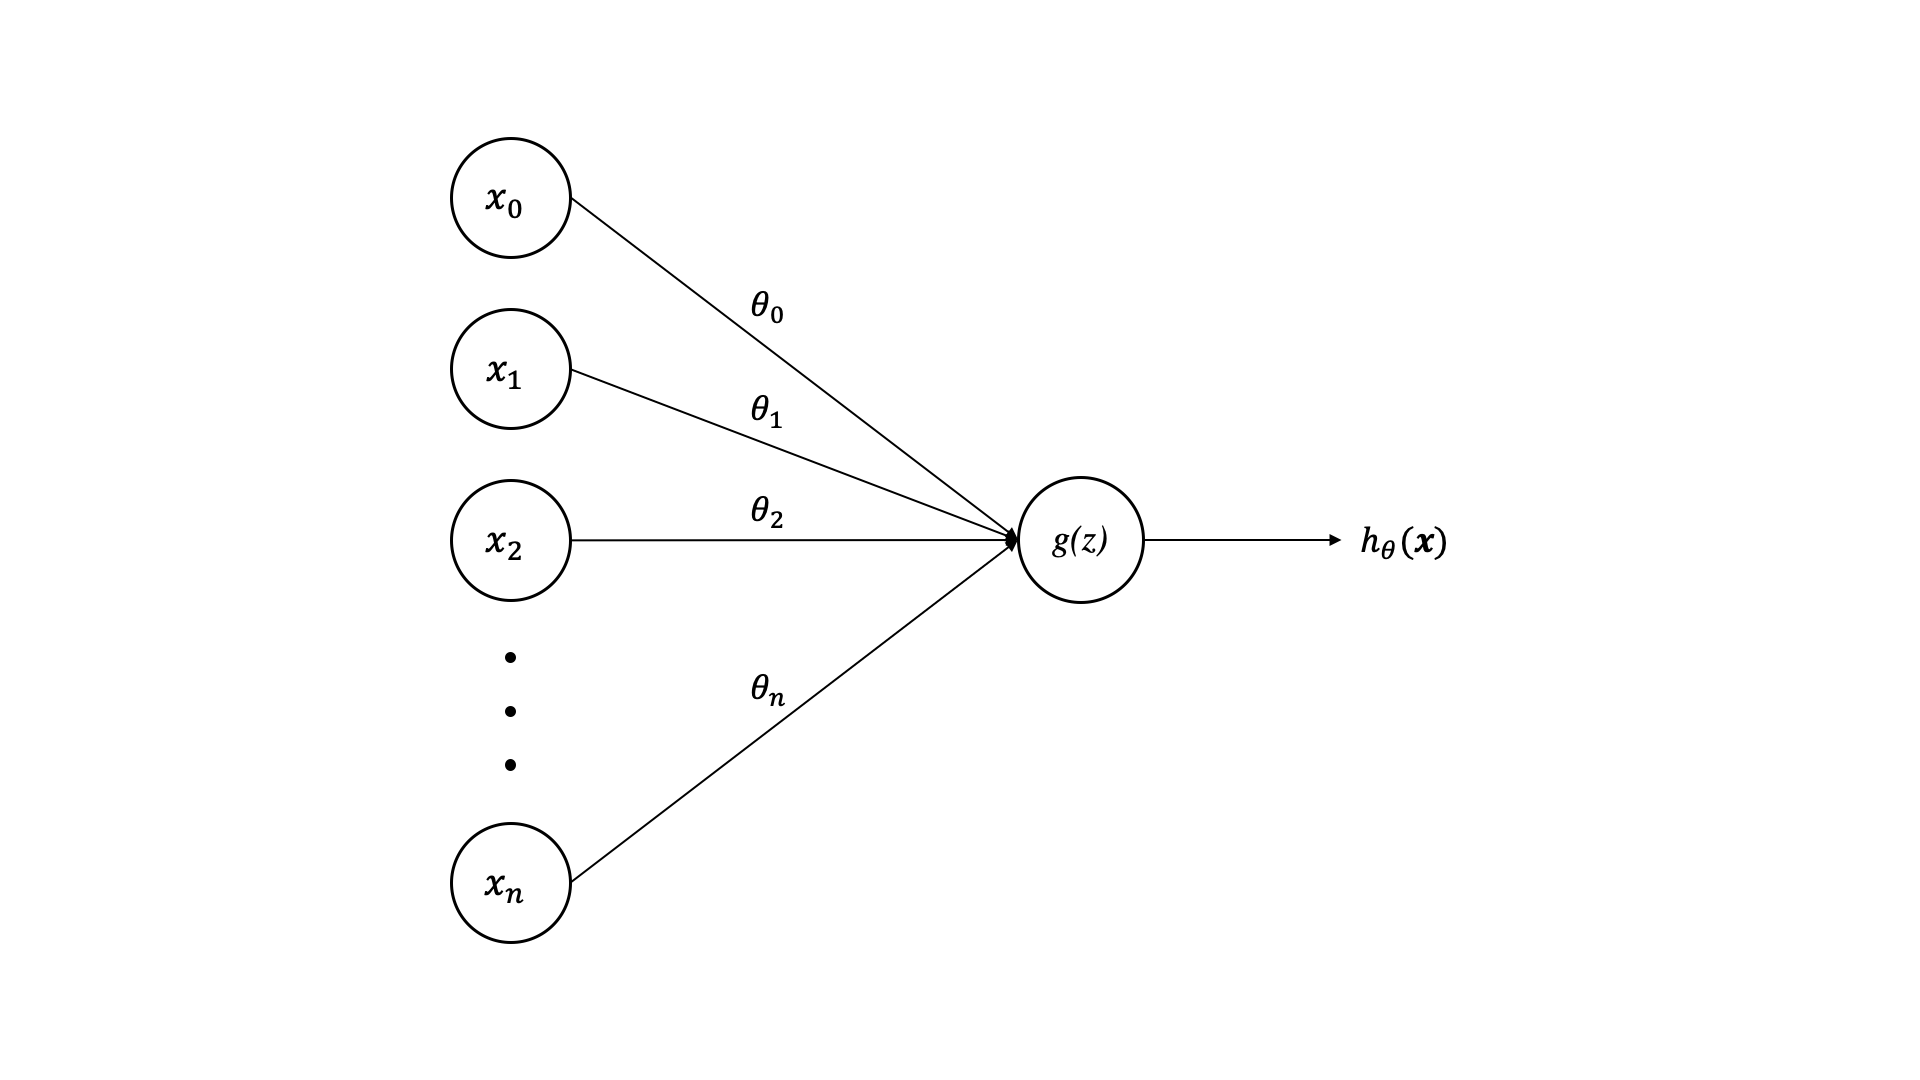
\includegraphics[width=0.7\textwidth]{figures/fitting/neuron_diagram.png}
    \caption{Diagram representation of a neuron}
    \label{fig:neuron_diag}
\end{figure}

In order to find the best weights $\btheta$, the error function is defined as we did in the previous section and it can be minimized with the gradient descent method. As it has been previously mentioned, a single neuron does not work well for complex non-linear processes. To be able to make predictions in those cases, a more complex system is required. 

Neural networks are built by using the outputs of various neurons as the inputs for other neurons, then building layers. The first one is called \textit{input layer}, the last one, \textit{output layer} and the layers in between are usually called \textit{hidden layers}. Usually, a neural network with a high number of layers will be able to perform more complex predictions but it will also take more time to train.
vaig a descansar 15 minutillos i me fico amb gd valis? vale andrea tranquila, tu descansa, eres la millor, best of the world
vale arnau, gracies per la teua comprensió
de res andrea, lo que necessites sempre
\begin{figure}[ht]
    \centering
    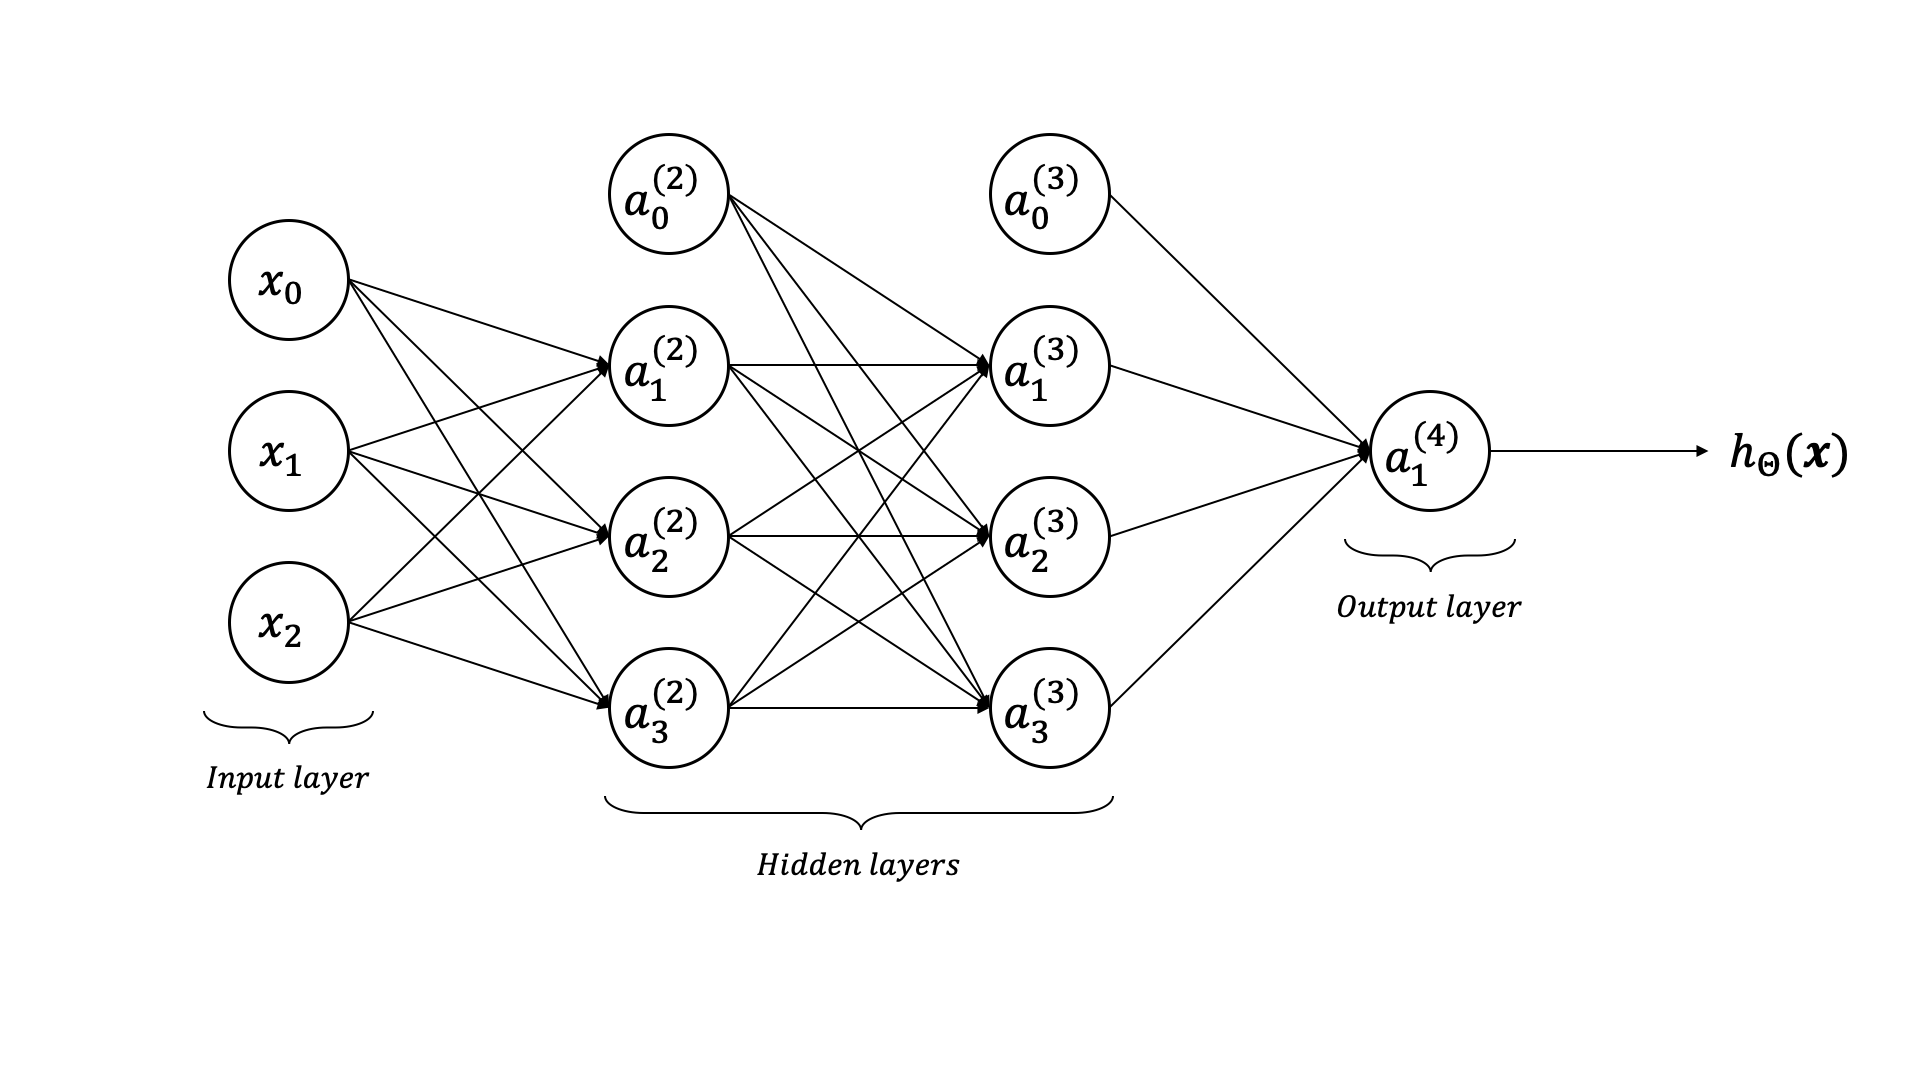
\includegraphics[width=0.7\textwidth]{figures/fitting/neural_network_example.png}
    \caption{Example of a neural network}
    \label{fig:neural_network_example}
\end{figure}

An example of a neural network is shown in Fig. \ref{fig:neural_network_example}. In this diagram, $a_i^{(j)}$ denotes the result of evaluating the activation function at the unit $i$ of the layer $j$. It is important to remark that $x_0$ and the activation values $a_0^{(j)}$, which are known as bias, are always set to 1. This is the reason why these nodes do not have any input. Also, we define $\bTheta^{(j)}$ as the matrix of weights controlling the function mapping from layer $j$ to $(j+1)$. The procedure to estimate $h_\Theta(\x)$, also known as forward propagation, consists on computing the activation $a_i^{(j)}$ at each one of the units in the neural network, starting from the input layer and moving forward to the output layer. This process is shown below for the example in the diagram of Fig. \ref{fig:neural_network_example}.

\begin{enumerate}
    \item Activation of layer 2
    \begin{equation}
    \begin{split}
        a_1^{(2)} &= g(z_1^{(2)}) = g(\bTheta_{10}^{(1)} + \bTheta_{11}^{(1)} x_1 + \bTheta_{12}^{(1)} x_2) \\
        a_2^{(2)} &= g(z_2^{(2)}) = g(\bTheta_{20}^{(1)} + \bTheta_{21}^{(1)} x_1 + \bTheta_{22}^{(1)} x_2) \\
        a_3^{(2)} &= g(z_3^{(2)}) = g(\bTheta_{30}^{(1)} + \bTheta_{31}^{(1)} x_1 + \bTheta_{32}^{(1)} x_2)
    \end{split}
    \end{equation}
    \item Activation of layer 3
    \begin{equation}
    \begin{split}
        a_1^{(3)} &= g(z_1^{(3)}) = g(\bTheta_{10}^{(2)} + \bTheta_{11}^{(2)} a_1^{(2)} + \bTheta_{12}^{(2)} a_2^{(2)} + \bTheta_{13}^{(2)} a_3^{(2)}) \\
        a_2^{(3)} &= g(z_2^{(3)}) = g(\bTheta_{20}^{(2)} + \bTheta_{21}^{(2)} a_1^{(2)} + \bTheta_{22}^{(2)} a_2^{(2)} + \bTheta_{23}^{(2)} a_3^{(2)}) \\
        a_3^{(3)} &= g(z_3^{(3)}) = g(\bTheta_{30}^{(2)} + \bTheta_{31}^{(2)} a_1^{(2)} + \bTheta_{32}^{(2)} a_2^{(2)} + \bTheta_{33}^{(2)} a_3^{(2)})
    \end{split}
    \end{equation}
    \item Activation of layer 3: prediction
    \begin{equation}\label{eq:nn_cost_function}
        h_\Theta(\x) = a_1^{(3)} = g(z_1^{(4)}) = g(\bTheta_{10}^{(3)} + \bTheta_{11}^{(3)} a_1^{(3)} + \bTheta_{12}^{(3)} a_2^{(3)} + \bTheta_{13}^{(3)} a_3^{(3)})
    \end{equation}
\end{enumerate}

The architecture of a neural network is mainly defined by the number of layers, the number of units in each layer and the activation functions that are used. The number of units of the input and output layers is usually restricted by the characteristics and goals of the application at hand. The number of input nodes is determined by the number of features that are used, since this layer is indeed used to feed the network with data. The number of output units can be larger than one and it is chosen depending on the type of problem that is confronted. For example, a classification problem requires as many output units as classes, so that the output of each unit $k$ represents the probability of the input example to pertain to the class $k$. 

The size of the hidden layers, both in terms of number of layers and number of units per layer, is generally a difficult part in the design of a neural network since there is no direct rule to decide among the different possibilities. Therefore, these are usually chosen by trial and error procedures. On the one hand, having too small hidden layers may lead to underfitting or even the inability of the algorithm to converge. On the other hand, having too large and/or too many hidden layers will increase the computation complexity and may also lead to overfitting \cite{aggarwal_neural_2018}. Nonetheless, a big majority of problems can be faced using a network with one hidden layer \cite{aggarwal_neural_2018}. Actually, it has been shown that a single hidden layer of nonlienar units and a single linear output layer can compute almost any "reasonable" function \cite{hornik_multilayer_1989}. Although this theoretical claim is not always easy to apply because it may require a huge amount of features.

The choice of the activation cost function is a critical decision in the design of a neural network. Any network with all the activation functions being linear will provide the same results as a Least Squares. In order to obtain more complex behavior, some unlinearities need to be added. To do so, many options of activation functions are proposed. The performanece of these different activation functions also depends on the type of problem that is being faced, but it usually requires some trial and error as well. Next, some examples of activation functions are shown.

\begin{itemize}
    \item Linear function
    \begin{equation}\label{eq:act_linear}
        g(z) = z
    \end{equation}
    \item Sigmoid function
    \begin{equation}\label{eq:act_sigmoid}
        g(z) = \frac{1}{1+e^{-z}}
    \end{equation}
    \item Tanh function
    \begin{equation}\label{eq:act_tanh}
        g(z) = \frac{e^{2z} - 1}{e^{2z} + 1}
    \end{equation}
    \item Rectifier Linear Unit (ReLU)
    \begin{equation}\label{eq:act_relu}
        g(z) = \max(0, z)
    \end{equation}
\end{itemize}



\subsection{Training a neural network}
Training a neural network is basically finding the weights for the $L$ layers, $\bTheta = \{\bTheta^{(1)}, \bTheta^{(2)}, ..., \bTheta^{(L)}\}$, that minimize the cost function of the neural network, which describes the error between the actual measurements and the predictions. This is

\begin{equation}
    \min_{\bTheta} J(\bTheta) = \min_{\bTheta} \frac{1}{2m} \left(\sum_{i=1}^{m} \left(y^{(i)} - h_\Theta (\x^{(i)}) \right)^2 \right) + \frac{\lambda}{2m} \sum_{l=1}^{L} \sum_{i=1}^{s_l} \sum_{j=1}^{s_{l+1}} (\bTheta_{j,i}^{(l)})^2
\end{equation}

where $m$ is the number of examples in the data set, $\lambda$ denotes the regularization term, and $s_l$ is the number of units of the layer $l$.

To obtain this minimum in $J(\bTheta)$ we use the gradient descent. The problem that we encounter is that, given the very high complexity of this cost function, we virtually cannot compute its gradient. This is where the backpropagation algorithm appears. This method allows to obtain the equivalent of the gradient for a neural network in a much more efficient way.

This algorithm starts with a random initialization of the parameters $\bTheta$. Then, it performs forward propagation with an example $(\x^{(i)}, y^{(i)})$ to obtain an estimation $h_\Theta(\x^{(i)})$. Once the estimation is obtained, the error of $h_\Theta(\x^{(i)})$ with respect to $y^{(i)}$ is obtained. This error is then "propagated" back in the network, so that we obtain a representation of the contribution of each node to the final error. This process is then repeated for each one of the examples given in the training set. The exact procedure of this algorithm is detailed next.

Given a training set $\set{(\x^{(1)}, y^{(1)}), (\x^{(2)}, y^{(2)}), ... (\x^{(m)}, y^{(m)})}$

\begin{enumerate}
    \item Set $\bDelta_{ij}^{(l)} = 0$ , $\forall l, i, j$
    \item Randomly initialize $\bTheta = \{\bTheta^{(1)}, \bTheta^{(2)}, ..., \bTheta^{(L)}\}$
    \item For $i$ from 1 to m:
    \begin{enumerate}[i.]
        \item Perform forward propagation to obtain $\ba ^{(l)}$ for $l=2, 3, ..., L$
        \item Calculate $\delta^{(L)} = a^{(L)} - y$
        \item For l from $(L-1)$ to 2:
        \begin{enumerate}[a.]
            \item $\bdelta^{(l)} = (\bTheta^{(l)})^T\bdelta^{(l+1)} \odot g'(\bz^{(l)})$\footnote{The symbol $\odot$ denotes the Hadamard or element-wise product}
        \end{enumerate}
        \item Update $\bDelta^{(l)}$ as $\bDelta^{(l)} := \bDelta^{(l)} + \bdelta^{(l+1)}(\ba^{(l)})^T$
    \end{enumerate}
    \item End for
    \item Calculate $\bD_{ij}^{(l)} = \frac{1}{m} \bDelta_{ij}^{(l)}$ if $j = 0$
    \item Calculate $\bD_{ij}^{(l)} = \frac{1}{m} \bDelta_{ij}^{(l)} + \lambda \bTheta_{ij}^{(l)}$ if $j \neq 0$
\end{enumerate}

The final result that we obtain after the backpropagation algorithm is equivalent to the gradient of the cost function of the neural network

\begin{equation}
    \bD_{ij}^{(l)} = \pdv{}{\bTheta_{ij}^{(l)}} J(\bTheta)
\end{equation}

% Overfit / Underfit (here?)

\subsection{Architecture of our neural network}
Given the nature of the neural networks, there exist an infinity of possibilities when trying to decide the architecture of a network. Nonetheless, it is usually a good practice to start with a simple design and then, if needed, move to more complex configurations. In our case we started with one hidden layer which has the same number of units as the input layer. This design is widely recommended as it has been found to perform well in a large variety of cases. Also, since we are dealing with a linear regression problem we need to have only one unit in the output layer.

The other defining characteristic of a neural network is the activation function that is used. On the one hand, we decided to use a ReLU activation function for the units in the hidden layer. This activation function has shown very good performance in linear regression problems. On the other hand, the output layer implements a linear activation function, because the possible output values that we can have for our problem are not bounded.

%==================================================================================================================

\chapter{Results} \label{ch:results}

%=================================================================================================================================================

\chapter{Conclusions}\label{ch:conclusions}

\clearpage
\printbibliography

\end{document}